\documentclass{article} % use option titlepage to get the title on a page of its own.
\usepackage{polski}
\usepackage[utf8]{inputenc}
\usepackage{graphicx}
\usepackage[a4paper, total={7in, 10in}]{geometry}
\usepackage{listings}
\usepackage{amsmath}
\graphicspath{ {./images/} }
\title{Rozwiązywanie układów równań liniowych}
\date{20.04.2018}
\author{Mateusz Buchajewicz}
\begin{document}
\maketitle

\section{Wprowadzenie}
Celem projektu jest implementacja metod iteracyjnych (Jacobiego i Gaussa-Seidla) i
bezpośrednich (Gaussa) rozwiązywania układów równań liniowych. Do implementacji wykorzystano język Python.

\section{Zadanie A}
Celem zadania było utworzenie układu równań:
\begin{equation}
\mathbf{Ax} = \mathbf{b}
\end{equation} 
Dla numeru indeksu 171619 otrzymujemy a1 = 6 i N = 54. \newline
Macierz \textbf{A} dla powyższych danych wygląda w ten sposób: \newline
\[
\textbf{A} = 
\begin{bmatrix}
    6 & -1 & -1 & 0 & 0 &\dots & 0 & 0 & 0 \\
    -1 & 6 & -1 & -1 & 0 & \dots & 0 & 0 & 0\\
    -1 & -1 & 6 & -1 & -1 & \dots & 0 & 0 & 0 \\
    0 & -1 & -1 & 6 & -1 & \dots & 0 & 0 & 0 \\
    \vdots & \vdots & \vdots & \vdots & \vdots & \ddots & \vdots & \vdots & \vdots \\
    0 & 0 & 0 & 0 & 0 & \dots & 6 & -1 & -1 \\
    0 & 0 & 0 & 0 & 0 & \dots & -1 & 6 & -1 \\
    0 & 0 & 0 & 0 & 0 & \dots & -1 & -1 & 6 \\
\end{bmatrix}
\]
Natomiast wektor \textbf{b} jest obliczany ze wzoru \( \mathbf{b_{i}} = sin(i*(f+1))\), co dla \(f = 9\) daje następujący wektor:
\[
    \textbf{b} = 
\begin{bmatrix}
    0.0 & -0.54402 & 0.91295 & -0.98803 & \dots & -0.99780 & 0.80112
\end{bmatrix}^T
\]
\section{Zadanie B}
W ramach tego zadania rozwiązano powyższy układ równań za pomocą metod iteracyjnych Jacobiego i Gaussa-Seidla. \\
\begin{center} 
    \begin{tabular}  { | l | c | r |   }
        \hline
        Metoda & Czas (s) & Liczba iteracji  \\
        \hline
        Jacobiego & 0.1027 & 67 \\
        \hline
        Gaussa-Seidla & 0.0618 & 40 \\
        \hline
    \end{tabular}
\end{center}
Iterację przeprowadzano, dopóki norma z wektora residuum była niemniejsza niż \(10^{-9}\).
\newpage
\section{Zadanie C}
W ramach tego zadania utworzono macierz \textbf{C} podobnie jak w zadaniu 1, przy czym a1 = 3. \\
Macierz \textbf{C} wygląda w ten sposób: \\
\[
\textbf{C} = 
\begin{bmatrix}
    3 & -1 & -1 & 0 & 0 &\dots & 0 & 0 & 0 \\
    -1 & 3 & -1 & -1 & 0 & \dots & 0 & 0 & 0\\
    -1 & -1 & 3 & -1 & -1 & \dots & 0 & 0 & 0 \\
    0 & -1 & -1 & 3 & -1 & \dots & 0 & 0 & 0 \\
    \vdots & \vdots & \vdots & \vdots & \vdots & \ddots & \vdots & \vdots & \vdots \\
    0 & 0 & 0 & 0 & 0 & \dots & 3 & -1 & -1 \\
    0 & 0 & 0 & 0 & 0 & \dots & -1 & 3 & -1 \\
    0 & 0 & 0 & 0 & 0 & \dots & -1 & -1 & 3 \\
\end{bmatrix}
\]
Próby obliczenia układu równań \(\mathbf{Cx}=\mathbf{b}\) 
za pomocą powyższych metod iteracyjncyh kończyły się pythonowym błędem "\textit{OverflowError - Result too large}" 
(odpowiednio po 1280 iteracjach metodą Jacobiego i 619 metodą Gaussa-Seidla),
z czego wnioskuję, że te metody iteracyjne dla takich wartości nie zbiegają się.
\section{Zadanie D}
W ramach tego zadania rozwiązano powyższy układ równań za pomocą
 metody bezpośreniej: faktoryzacji LU. 
W tym przypadku norma z residuum wyniosła około \(1.8956*10^{-15}\),
 co oznacza wysoką dokładność wykonanych obliczeń.
\section{Zadanie E}
W ramach tego zadania utworzono wykres zależności czasu od ilości iteracji dla powyższych metod. Zależność została przedstawiona na poniższym wykresie:
\begin{figure}[h]
    \centering
    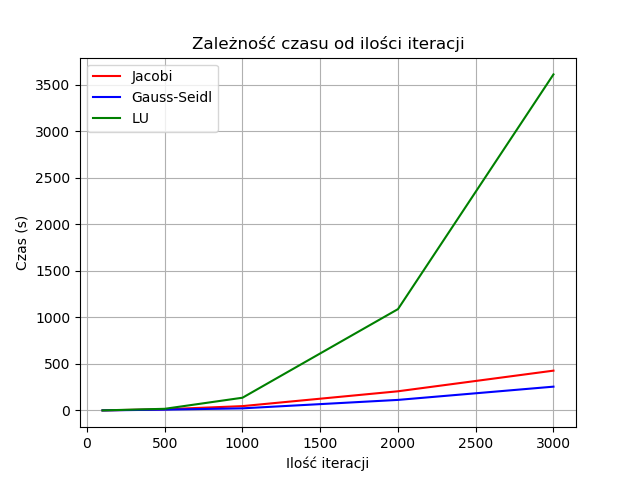
\includegraphics[scale=0.7]{wykres.png}
    \caption{ wykres zależności czasu od ilości iteracji dla metod Jacobiego, Gaussa-Seidla i LU}
\end{figure}
\section{Zadanie F}
Oczekiwanie na wygenrowanie wykresu, wtedy będą wnioski.
\end{document}